% additional use of \usepackage{beamerthemesplit}
\documentclass{beamer}
\usepackage{beamerthemesplit} % new 
\usepackage{hyperref}
\usepackage{multimedia}
\usepackage[spanish]{babel}
\usetheme{Frankfurt}
\definecolor{verde}{rgb}{0,0,1}
\definecolor{rojo}{rgb}{1,0,0}
\definecolor{vio}{rgb}{0.5,0,0.5}
\definecolor{rosa}{rgb}{0.8,0.1,0.1}
\newcommand{\director}{Collaborators:\\ Mart\'{\i}n de los R\'{\i}os \& Dante Paz}

\begin{document}
\title{Merging Systems Identification in Systems of Galaxies.} 
\author{Mariano J. Dom\'{\i}nguez R.\inst{1}, \\
 Mart\'{\i}n de los R\'{\i}os\inst{1} \& Dante Paz\inst{1}}
\institute[IATE and others]
{
  \inst{1}%
  IATE-OAC-CONICET
  \and
  \vskip-2mm
}

\date[VLC 2013] % (optional)
{GG2014Conference, November 2014}

\logo{
\includegraphics[height=1.5cm]{logo_iate_nuevo_trans.jpg}}

\frame{\titlepage

} 

\frame{
\tableofcontents} 


\section{Motivation.}
\frame{
\tableofcontents[ 
    currentsection, 
    hideothersections, 
    sectionstyle=show/hide, 
    sectionstyle=show/shaded, 
    ] 
}

\frame{\frametitle{Motivation:}
\begin{itemize}
\item The nature of dark matter is still a \alert{great unsolved astrophysical problem (EoS of DM, GR in GG)}.
\item Laboratory searches for the DM candidates succeeded in showing that any interaction
 between the dark and baryonic matter is vanishingly small (CDMS, XENON, PANDAX, etc).
\item Despite their size, galaxy clusters have an average projected
mass density of order $0.1 - 1 g cm^{-2}$, so they are no match for
the laboratory experiments for constraining the DM-baryon interactions.
\item However, clusters and galaxies may provide the
best available laboratory for studying the DM self-interaction.
\end{itemize}
}

\frame{\frametitle{Markevicht et al 2004:}
\begin{itemize}
 \item Studing the dinamics of merging clusters allow us determinate some properties of dark matter particles,
since provide a diagnostic of large scale structure (LSS) formation.
 \item Provide empirical evidence favoring DM over modified gravity (Clowe et al. 2006).
\end{itemize}

\begin{alertblock}{Important for this work}
provide constraints on the DM self-interaction cross-section in three different ways as follows:
\end{alertblock}
}


\subsection{The Bullet Cluster.} 

\frame{\frametitle{The Bullet Cluster}
\begin{tiny}
\begin{columns}
 \begin{column}{4cm}
  \begin{itemize}
  \item Optical Image.
   \item {\color{pink} X-ray emission of the ICM.}
   \item {\color{blue} Estimated mass using WL.}
  \end{itemize}
 \end{column}
\begin{column}{7cm}
\begin{figure}
 \centering
 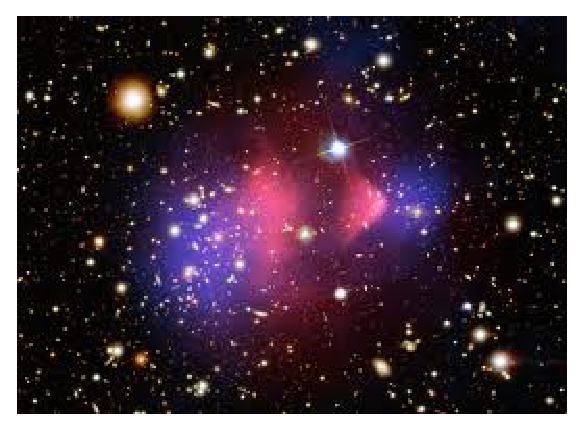
\includegraphics[scale=0.8]{./bullet.eps}
\end{figure}
\end{column}
\end{columns}
\end{tiny}

The most remarkable feature  is a ∼ 23" offset between the subcluster’s DM centroid 
and the gas bullet, which is at least 2$\sigma$ significant.

}

\frame{\frametitle{The gas -- Dark Matter offset:}
\begin{itemize}
 \item The offset between the subcluster’s DM centroid and the gas bullet, means that the scattering depth $\tau$
  of the dark matter subcluster w.r.t. collisions with the flow of dark matter particles cannot be much 
  greater than 1: $ \tau_{s}=\frac{\sigma}{m} \Sigma_{s} $ 
\end{itemize}

where $\sigma$ is the DM collision cross-section, \textit{m} is its particle mass and $\Sigma_{s}$ is the 
DM surface density of the subcluster.  The surface density averaged over the face of the subcluster is
$\Sigma \approx 0.2 g cm^{-2}$. Assuming spherical symmetry and requiring that $\tau_{s}<1$, we obtain
$\frac{\sigma}{m} < 5 cm^{2}g^{-1}$. \alert{See also Merging Cluster Colaboration}.
\begin{table}
\begin{tabular}{|c|c|}
\hline
 Cluster & $\frac{\sigma}{m}$ \\
 \hline \hline
 Bullet Cluster & $< 5 cm^{2}/g$ \\
 Musket Ball & $<7 cm^{2}/g$ \\
 Baby Bullet & $<4 cm^{2}/g$ \\
\hline
 \end{tabular}
 \end{table}

}

\frame{\frametitle{The high velocity of the subcluster and its survival:} 

\begin{eqnarray}
    v-v_{ff} & = & \frac{\bar{p}}{m}\frac{\sigma}{m} \Sigma_{m} \\
    v-v_{ff} &<& 1000 km/s \\
    \frac{\sigma}{m} & < & 7cm^{2}/g
\end{eqnarray}
Its possible to put an upper limit on the integrated mass loss and thereby
 on the collision cross-section:
\begin{eqnarray}
 \chi&=&1-2\frac{v^{2}_{esc}}{v_{0}^{2}} \\
    \chi \tau_{m}&=&\frac{\sigma}{m}\Sigma_{m} \left[ 1-2 \frac{v_{esc}^{2}}{v_{0}^{2}} \right] \\
    \chi \tau_{m}&<&0.3 \\
    \frac{\sigma}{m}& < &1 cm^{2}/g
\end{eqnarray}
}

\frame{\frametitle{A problem for the $\Lambda$CDM cosmological model?}
\begin{itemize}
 \item Several works indicate that is very difficult to observe a cluster colllision with similar velocity:
    \begin{itemize}
%\begin{tiny}
    \item Hayashi et al. 2006
    \item Farrar and Rosen 2007
    \item Lee and Komatsu 2010
    \item Forero-Romero et al. 2010
    \item Thompson and Nagamine 2011
    \item Watson et al. 2013
%\end{tiny}
    \end{itemize}
 
 \item Studies using hydrodinamical simulations.
    \begin{itemize}
%\begin{tiny}
     \item Springel \& Farrar. 2005
     \item Milosavljevic et al. 2007
     \item Mastropietro \& Burket. 2008
     \item Lage and Farrar. 2014
%\end{tiny}
    \end{itemize}
 \item \alert{It should be recalled that the ICs parameter space is very large.}
\end{itemize}

}

\subsection{The Rise and Fall of a challenger (Thompson 2014).}
\frame{\frametitle{The Rise and Fall of a challenger by Thompson (2014).}
\begin{itemize}
\item They investigate the probability of finding such a high-velocity pair in 
large-volume N-body simulations, particularly focusing on differences between halo finding algorithms.
\item  When employing the Rockstart (Behroozi et al 1013) halo finder that considers particle velocities, they find
numerous Bullet-like pair candidates that closely match not only the high pairwise velocity, 
but also the mass, mass ratio, separation distance, and collision angle that have been shown to produce the Bullet Cluster.
\item The probability of finding a massive, high pairwise velocity pair
among halos with $M_{\rm halo}\geq10^{14} M_\odot$ is $4.6\times 10^{-4}$
using \RS, while it is $\approx 45\times$ lower using a friends-of-friends (FOF) based approach as in previous studies.
\end{itemize}
}


\frame{\frametitle{High velocity tail of Bullet like pairs.}
\begin{figure}[h!]
 \centering
 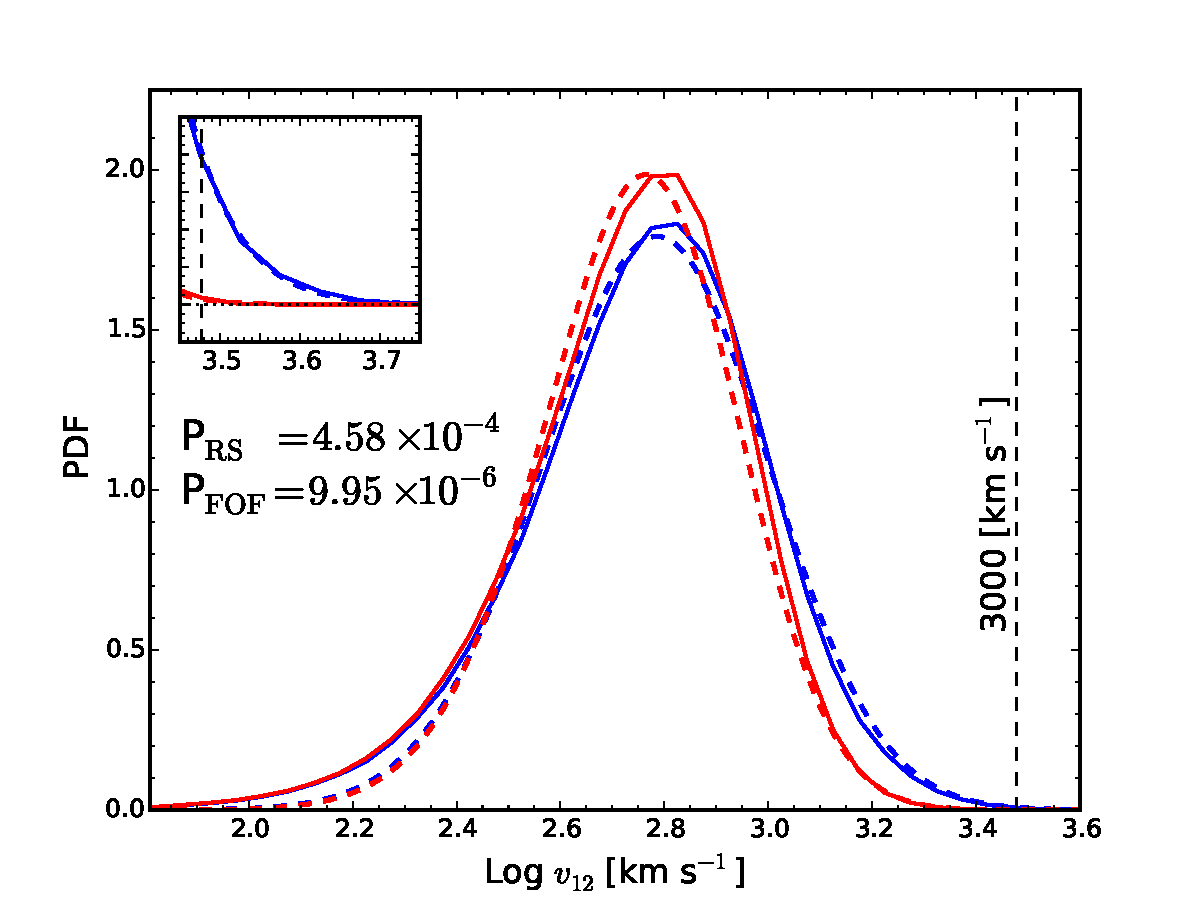
\includegraphics[scale=0.3]{./figure3.pdf}
 % mill.png: 555x565 pixel, 72dpi, 19.58x19.93 cm, bb=0 0 555 565
 \caption{Probability distribution function of massive halo pairs (M$_{12}\geq10^{14}\Msun, d_{12}\leq10\rm{Mpc}$) in 
largest simulation (L4500) identified by FOF (Red solid line) and RS (Blue solid line).}
\end{figure}
}


\section{Mock galaxy catalogs.}

\frame{
\tableofcontents[ 
    currentsection, 
    hideothersections, 
    sectionstyle=show/hide, 
    sectionstyle=show/shaded, 
    ] 
}

\subsection{Millenium Simulation (Springel et al. 2005).}


\frame{\frametitle{Simulaci\'on Millenium}
\begin{figure}[h!]
 \centering
 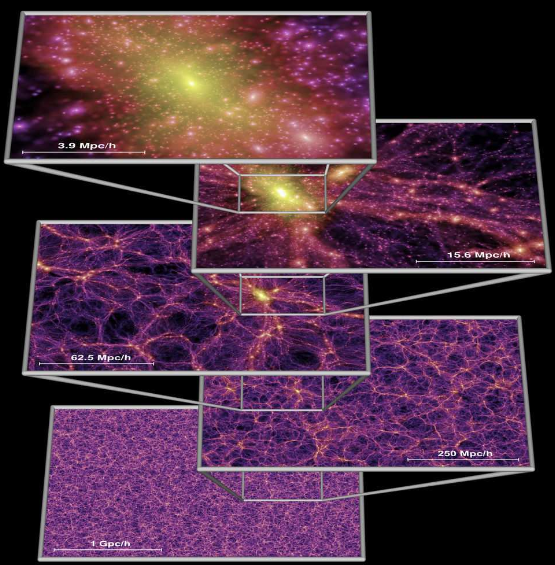
\includegraphics[scale=0.3]{./mill.png}
 % mill.png: 555x565 pixel, 72dpi, 19.58x19.93 cm, bb=0 0 555 565
 \caption{$\Lambda$CDM model (Ruiz et al 2012) + gadget3 + FoF/SubFind}
\end{figure}
}


\frame{\frametitle{Using the Merging Trees Information.}
\begin{itemize}
 \item Starting from the subhalos merging trees, we build up the FoF groups merging trees.
\alert{but we are actually running new simulations and making its merging trees using consistent trees!}
\end{itemize}

\begin{figure}[h!]
 \centering
 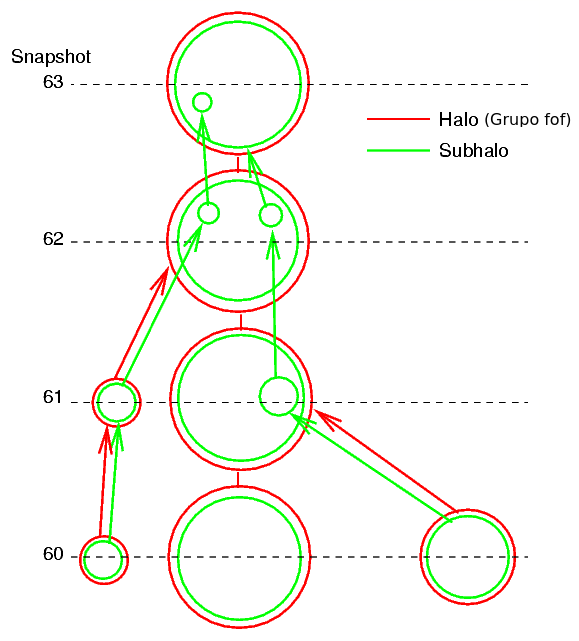
\includegraphics[scale=0.32]{./tree.png}
 % tree.eps: 0x0 pixel, 300dpi, 0.00x0.00 cm, bb=14 14 554 655
\end{figure}

}

\subsection{Semi-analytic model: (Guo 2010).}

\frame{\frametitle{Buil up of mock catalogs:}
We simulate the local SDSS universe ($4 \pi$, $z<0.12$) with SDSS-DR7 angular mask, replicating 
the MS box.

\begin{columns}
 \begin{column}{4.2cm}
  \begin{figure}[h!]
 \centering
 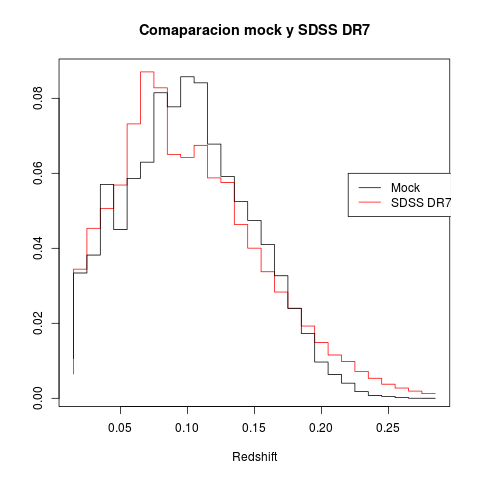
\includegraphics[scale=0.31]{./comparacion_red.png}
 % comparacion_red.png: 480x480 pixel, 72dpi, 16.93x16.93 cm, bb=0 0 480 480
\end{figure}
 \end{column}
 \begin{column}{5cm}
  \begin{figure}[h!]
 \centering
 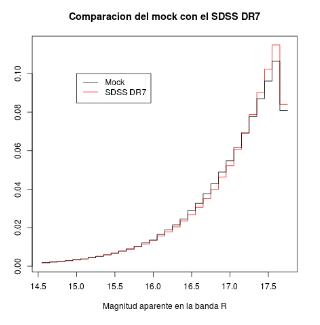
\includegraphics[scale=0.45]{./nu.png}
 % comaracion_bandar.png: 480x480 pixel, 72dpi, 16.93x16.93 cm, bb=0 0 480 480
\end{figure}
 \end{column}
\end{columns}
}

\section{Looking for substructures in systems of galaxies:}
\frame{
\tableofcontents[ 
    currentsection, 
    hideothersections, 
    sectionstyle=show/hide, 
    sectionstyle=show/shaded, 
    ] 
}

\subsection{Dressler-Shectman Test (1988):}
\frame{\frametitle{Dressler-Shectman Test (1988):}
\begin{itemize}
 \item Introducing the estimator: $\delta^{2}=(\frac{11}{\sigma^{2}})[(v_{local}-v)^{2}+(\sigma_{local}-\sigma)^{2}]$
where \pause
 \item $v$: mean velocity of the cluster. 
 \item $v_{local}$: mean local velocity.  Computed using the 10 nearby neighbours. 
 \item $\sigma$: cluster velocity dispersion. 
 \item $\sigma_{local}$: local velocity dispersion. 
 \item For systems just add: $\Delta=\Sigma\delta$. 
 \item \textit{Pinkney et al. (1996)} 
  

  \begin{itemize}
 \begin{tiny}
   \item Best test for substructures identification.
   \item Low effectivity when the substructures yield along los and when the cluster occupacy is lower than 30 gx.
   \item Recommended to be complemented  with Skewness measurements of the distribution of radial velocities. 
   \item Can identify substructures 3 Gyr before the merger, equivalent to ten snapshots in the MS.
 \end{tiny}
  \end{itemize}
\end{itemize}
}


\frame{
\begin{itemize}
 \item Since the underlying distribution of $\Delta$ is unknown, is neccesary run Monte Carlo realizations distribuying
randomly the velocities, in order to "erase" the substructures but conserving the global velocity distribution. \pause
 \item computing the p value as:
 
 \begin{equation}
  p=\frac{N(\Delta_{MC}> \Delta)}{N_{MC}}
 \end{equation}

 \item we select galaxies with a high probability of membership to subhaloes.

\end{itemize}
\begin{examples}
 Currently we turned to a machine learning methodology that select the galaxies in subhaloes based on a set of features, 
the most important ones are: $\delta$, $\Delta$, skewness of velocity distribution, color, magnitude and its correlations. Avoiding
the systems catalog. 
\end{examples}
}

\subsection{Mixture of Gaussians.}
\frame{\frametitle{Mixture of Gaussians (\textit{Mclust in R})}
Given that the application of the DS test leave us a subset of gaalxies with high probability
of reside in substructures, we join them in order to define the substructures and its physical 
properties: barycenter, virial radius, velocity dispersion, occupacy etc.

\begin{figure}[h!]
 \centering
 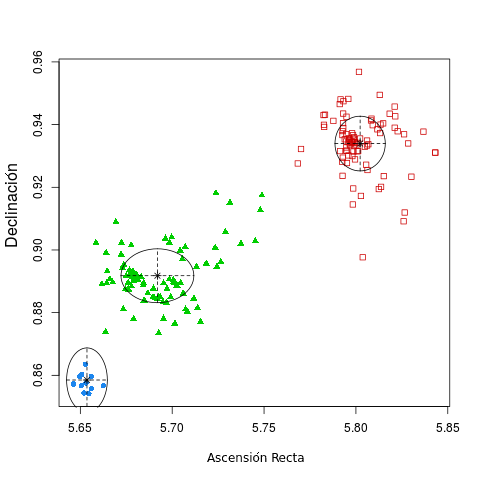
\includegraphics[scale=0.28]{./mclust_class.png}
 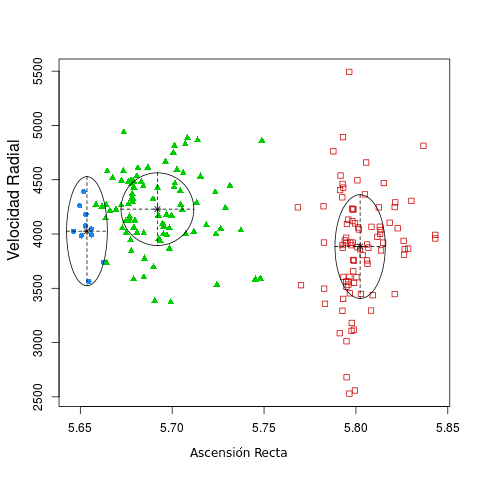
\includegraphics[scale=0.28]{./mclust_13.png}
 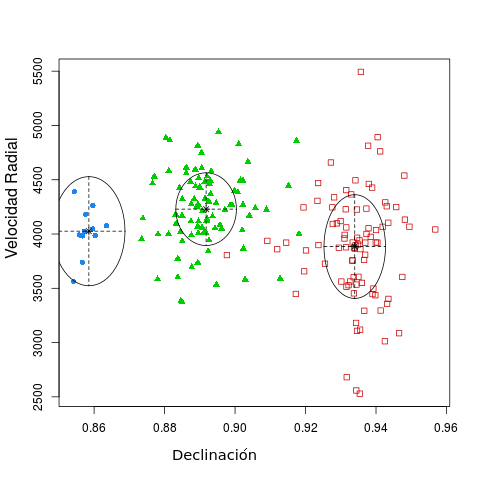
\includegraphics[scale=0.28]{./mclust_23.png}
 % mclust_class.png: 480x480 pixel, 96dpi, 12.70x12.70 cm, bb=0 0 360 360

\end{figure}
}


\frame{\frametitle{Aplication of the DS test in the simulated catalog}
\begin{itemize}
\item We apply the test to 2854 clusters with mass over $10^{13}M_{\odot}$ and more than 30 members in the mock catalog. 
\item Finding that 1448 clusters present subestructures ($p<0.15$), wich represent approximately over $50 \%$ of the sample. 
\item If aditionally ask that the skewness of the distribution of radial velocities different of 0, the sample reduces to 715 clusters.
\end{itemize}
}

\frame{\frametitle{We also introduce a iterative DS test}
\begin{itemize}
 \item We apply the iterative DS test to the 2854 cluster sample and found only 119 where the test converge. 
 \item Just 46 of this 119 systems of galaxies where detected using the traditional DS test complemented with the Skewnes test.
\end{itemize}

\begin{figure}[h!]
 \centering
 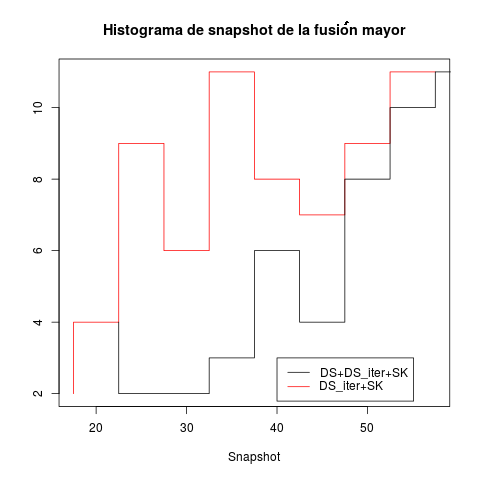
\includegraphics[scale=0.4]{./hist_snap_todo.png}

\end{figure}
}


\frame{\frametitle{Application of the mixture of Gaussians algorithm.}
\begin{itemize}
 \item Using \textit{Mclust} on the galaxies with $\delta > 2$. 
 \item leave 636 clusters, of 715 clusters, where inhabit 2 substructures with more than 5 members. 
 \item In general one of this substructures correspond to the cluster core or the most massive component of the merger. 
 \item Sometimes we found systems with problems in the groups parent catalog solved if we take into account the survey angular mask.
 \item After the substructure identification using Mclus, each one was associated with the corresponding halo using the galaxy members
 voting on the underlying halo catalog.  
\end{itemize}

}

\frame{\frametitle{Properties of the identified substructures:}
\begin{itemize}
\item  We compute the barycenter coordinates weigthed by luminosity in order to improve this determination. 
\item Resulting in good estimations of the geometrical centers of the subhalos using the galaxy members. 
\item After that we calculate the velocity dispersions and virial radius using:
 
\begin{eqnarray} \label{rvir_disp}
 R_{vir} & = & \frac{\pi}{2} \frac{ngal(ngal-1)}{\sum_{i>j}^{ngal}R_{ij}^{-1}} \nonumber\\
 \sigma &=& \frac{\sqrt{\pi}}{ngal(ngal-1)} \sum_{i=1}^{ngal-1} \omega_{i} g_{i} \nonumber\\
 \omega_{i} &=& i(ngal-i) \nonumber\\
 g_{i} &=& v_{i+1}-v_{i} \nonumber\\ 
\end{eqnarray}

\end{itemize}
}

\frame{\frametitle{Angular and velocity normalized difference positions.}

\begin{columns}
 \begin{column}{5cm}
\begin{figure}[h!]
 \centering
 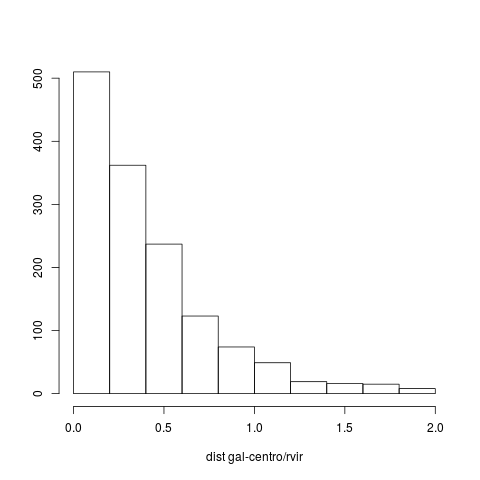
\includegraphics[scale=0.35]{./histo_dist_gal_centro.png}
\end{figure}
 \end{column}
 \begin{column}{5cm}

\begin{figure}[h!]
 \centering
  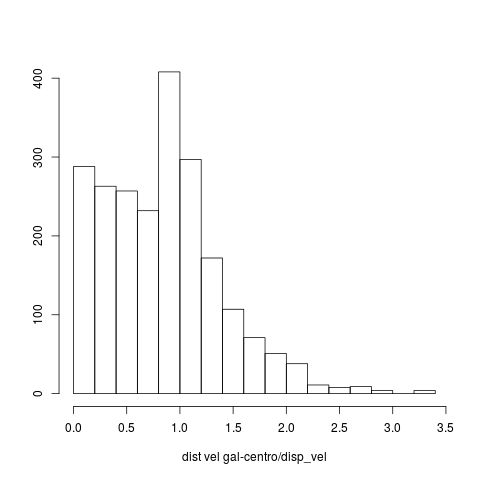
\includegraphics[scale=0.35]{./histo_distvel_gal_centro.png}
\end{figure}
 \end{column}
\end{columns}
}

\frame{\frametitle{Properties of the identified substructures:}
\begin{itemize}
 \item The velocity dispersion determinations results comparable with the real halo values.
 \item If we consider as substructure members those galaxies with a projected angular distance below one virial radius $r_{vir}$  and a radial 
velocity ofset lower than $2\sigma$. The mass determinations improve specially for the substructures (halo types=1). 
\end{itemize}

\begin{figure}[h!]
 \centering
 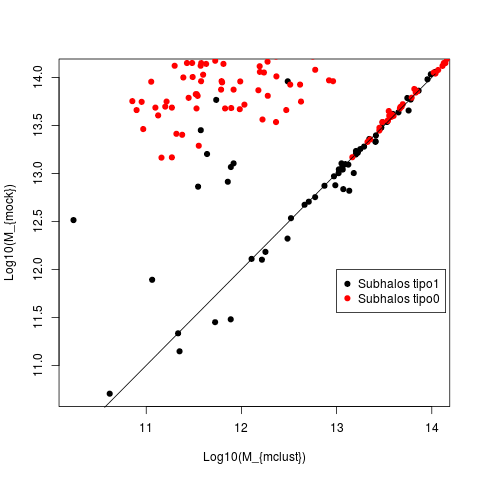
\includegraphics[scale=0.27]{./puto.png}
\end{figure}
}

\subsection{Controlling the projections effects.}
\frame{\frametitle{Region where los projections introduce errors:}

\begin{figure}[h!]
 \centering
 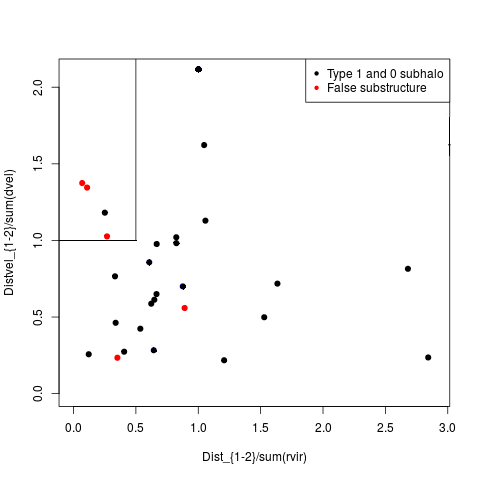
\includegraphics[scale=0.35]{./distancias.png}
 \caption{Projected distance between centers of groups identify with MG, normalized to the sum of the virial radius vs
 the difference in radial velocity normalized to the sum of the radial velocity dispersion. The black/red dots correspond
 to the clusters where we found the type 0 subhalo and a type 1 subhalo, and to the clusters where a false substructure 
 is identified respectively.}
\end{figure}

}

%------------------------------------------------------------------------------------------------------------------------------------------------
%------------------------------------------------------------------------------------------------------------------------------------------------
%------------------------------------------------------------------------------------------------------------------------------------------------
%------------------------------------------------------------------------------------------------------------------------------------------------
%------------------------------------------------------------------------------------------------------------------------------------------------
%------------------------------------------------------------------------------------------------------------------------------------------------
%------------------------------------------------------------------------------------------------------------------------------------------------
\section{Results.}
\frame{
\tableofcontents[ 
    currentsection, 
    hideothersections, 
    sectionstyle=show/hide, 
    sectionstyle=show/shaded, 
    ] 
}

\subsection{Bayesian merging systems geometry reconstructions.}
\frame{\frametitle{Dawson (2013) Bayesian reconstruction techniques in
 order to recover the 3D merger configuration.}

\begin{figure}[h!]
 \centering
 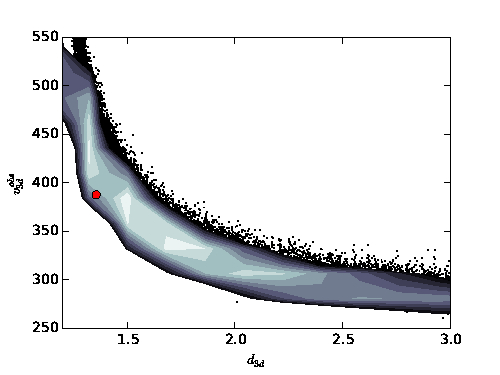
\includegraphics[scale=0.4]{./d_3d-vs-v_3dcol.jpg}
 \caption{Distribution of posterior probability in the 3D distance (Mpc) and 
3D velocity (Km/s) space for a simulated merging cluster, red dot indicates the real current values.
Others kinematical parameters like Time since Collision or velocity at the merger time are also well 
recovered.}
\end{figure}
}

\subsection{Application to the catalogs of systems of galaxies in SDSS and 2dF.}
\frame{\frametitle{Application to catalogs of systems of galaxies.}
\begin{itemize}
 \item Berlind et al (2008) include information on 8148 systems of galaxies, with 44554 galaxy members. 
 \item We identify the substructures present in clusters applying MG over all galaxies with $\delta>2$, we 
  found 2 significant substructures in $15$ clusters of the sample.
 \item Tempel et al (2012) include information in FoF 77858 clusters and groups of galaxies, with 576493 galaxy members.
 \item We found two significant substructures in $80$ clusters of the sample.
 \item Eke et al 2PIGGS catalog include information on 28877 clusters and grups of galaxies,  with 191440 galaxy members.
 \item We found two significant substructures in $38$ clusters of the sample.
\end{itemize}
}

\subsection{Hidden compact groups in the clusters?}
\frame{\frametitle{Hidden compact groups in clusters of galaxies?}
\begin{figure}[h!]
\centering
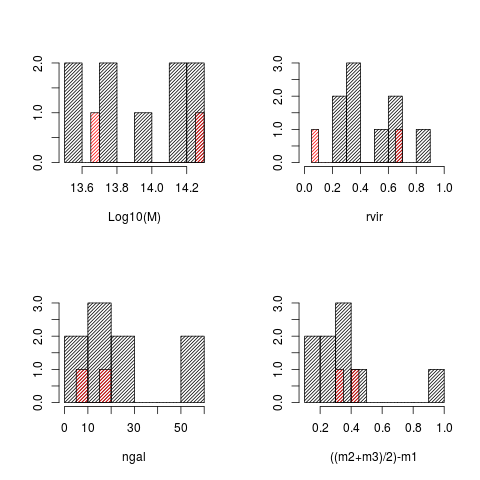
\includegraphics[scale=0.35]{./sub_prop.png}
\caption{Mass, virial radius (Mpc), halo occupation, and magnitude gap distributions of subhaloes identified on mock catalogs,
Two of this systems have a magnitude gap over 1 magnitude and virial radius $\sim 0.3$Mpc, }
\end{figure}
}

%\subsection{Comparaci\'on con otros resultados.}
%\frame{\frametitle{Comparaci\'on con otros resultados.}

%}
%------------------------------------------------------------------------------------------------------------------------------------------------
%------------------------------------------------------------------------------------------------------------------------------------------------
%------------------------------------------------------------------------------------------------------------------------------------------------
%------------------------------------------------------------------------------------------------------------------------------------------------
%------------------------------------------------------------------------------------------------------------------------------------------------
%------------------------------------------------------------------------------------------------------------------------------------------------
%------------------------------------------------------------------------------------------------------------------------------------------------

\section{Conclusions and Current work.}
\frame{
\tableofcontents[ 
    currentsection, 
    hideothersections, 
    sectionstyle=show/hide, 
    sectionstyle=show/shaded, 
    ] 
}

\frame{\frametitle{Conclusions:}
\begin{itemize}
\item We build up mock galaxy systems catalogs.
\item We study different methods of substructures identification, including a new iterative DS test. 
\item Using the merging tres information we recover the merging systems and its properties using as input a catalog of a systems of galaxies. 
\item We identify the substructures present in merging clusters, finding its member galaxies and computing its more relevant physical properties. 
\item Using this information we succesfully apply Bayesian methods of merger reconstruction in selected systems. 
\item We apply our methodology to real galaxy catalogs and provide a sample of over 100 low redshift merging (relaxed) systems of galaxies in different
 stages of the merging process.
\end{itemize}
}

\frame{\frametitle{Current Work:}
\begin{itemize}
 \item Develop a machine learning (LR, SVM, RF) subhalos identification algorithm using as training set the mock catalogs and K-Folds cross-validation.
 \item Calibrate the method developed using the new simulated catalogs in order to apply to intermediate/high redshift catalogs. 
 \item Study the physical properties of the galaxies (sSFR, Metallicity, HI abundance, morphologies) in the merging clusters (relaxed) and its 
 substructures. 
 \item Recently Gastaldello (2014) reported the first bullet group in the Strong Lensing Legacy Survey (SL2S), therefore we eliminate the restriction 
  of a minimum of 30 member galaxies in the parent catalog.
 \item Apply the astrophysical test over the merging cluster systems identified in order to determinate dark matter particles properties, 
including WL mass determinations information. 
\end{itemize}
}

\frame{
\begin{figure}[h!]
 \centering
 
\includegraphics[scale=0.4]{./gracias.png}
 % gracias.png: 657x518 pixel, 72dpi, 23.18x18.27 cm, bb=0 0 657 518
\end{figure}
}
\end{document}

